\subsection{Overall performance}\label{sec:main-results}

\begin{figure*}[t]
\centering

\includegraphics[width=0.85\textwidth]{figures/proxy_holdout_fullstage.pdf}
\caption{Proxy prediction versus ground-truth mIoU on the 27 held-out subsets
(54 scored runs: sibling-anchor and known-bad configuration per subset). Each
point is one pipeline run scored by the frozen lean proxy; the dashed line
marks the alarm threshold $\tau = 0.495$. Runs below the threshold are flagged
as low quality. Colours indicate lining family.}
\label{fig:holdout-scatter}
\end{figure*}

Before assessing the proxy on held-out tunnels, we verified its calibration on
the 120 exploration trials. The frozen lean model reaches a training MAE of
0.129 and Spearman rank correlation $\rho = 0.853$ ($n = 120$;
Fig.~\ref{fig:proxy-training}). A permutation control confirms the learned
relationship is genuine: refitting on label-shuffled trials yields MAE
$0.271 \pm 0.009$ over 20 repeats, well outside the real model's error.
Leave-one-family-out cross-validation gives MAE 0.156 and $\rho = 0.717$,
indicating that the feature--quality relationship transfers across families
rather than memorising any single anchor.

\begin{table}[ht]
\caption{Proxy fidelity on the 27 held-out subsets (54 scored runs; frozen
lean model).}\label{tab:holdout-fidelity}
\begin{tabular*}{\tblwidth}{@{} l c c @{}}
\toprule
Metric & Full-stage & v2 reference \\
\midrule
Spearman $\rho$ & 0.848 & 0.810 \\
MAE (overall) & 0.071 & 0.071 \\
MAE (staggered) & 0.071 & 0.067 \\
MAE (continuous) & 0.064 & 0.066 \\
MAE (complex) & 0.076 & 0.080 \\
Bad-run flagging & 27/27 TP, 0/27 FP & 27/27 TP \\
\bottomrule
\end{tabular*}
\end{table}

\textbf{Predictiveness and calibration on held-out tunnels.}
Table~\ref{tab:holdout-fidelity} and Fig.~\ref{fig:holdout-scatter} summarise
deployment-time fidelity. Across the 27 held-out subsets (54 scored runs),
none of which contributed to calibration, the proxy ranks runs with
$\rho = 0.848$ and predicts absolute mIoU to within 0.071 on average.
Calibration is stable across families (MAE 0.064--0.076), supporting the
single-pooled-model design: one unified proxy serves staggered, continuous,
and complex tunnels with per-family errors within 0.012 of each other, so no
per-family recalibration is required at deployment.

\begin{figure*}[t]
\centering
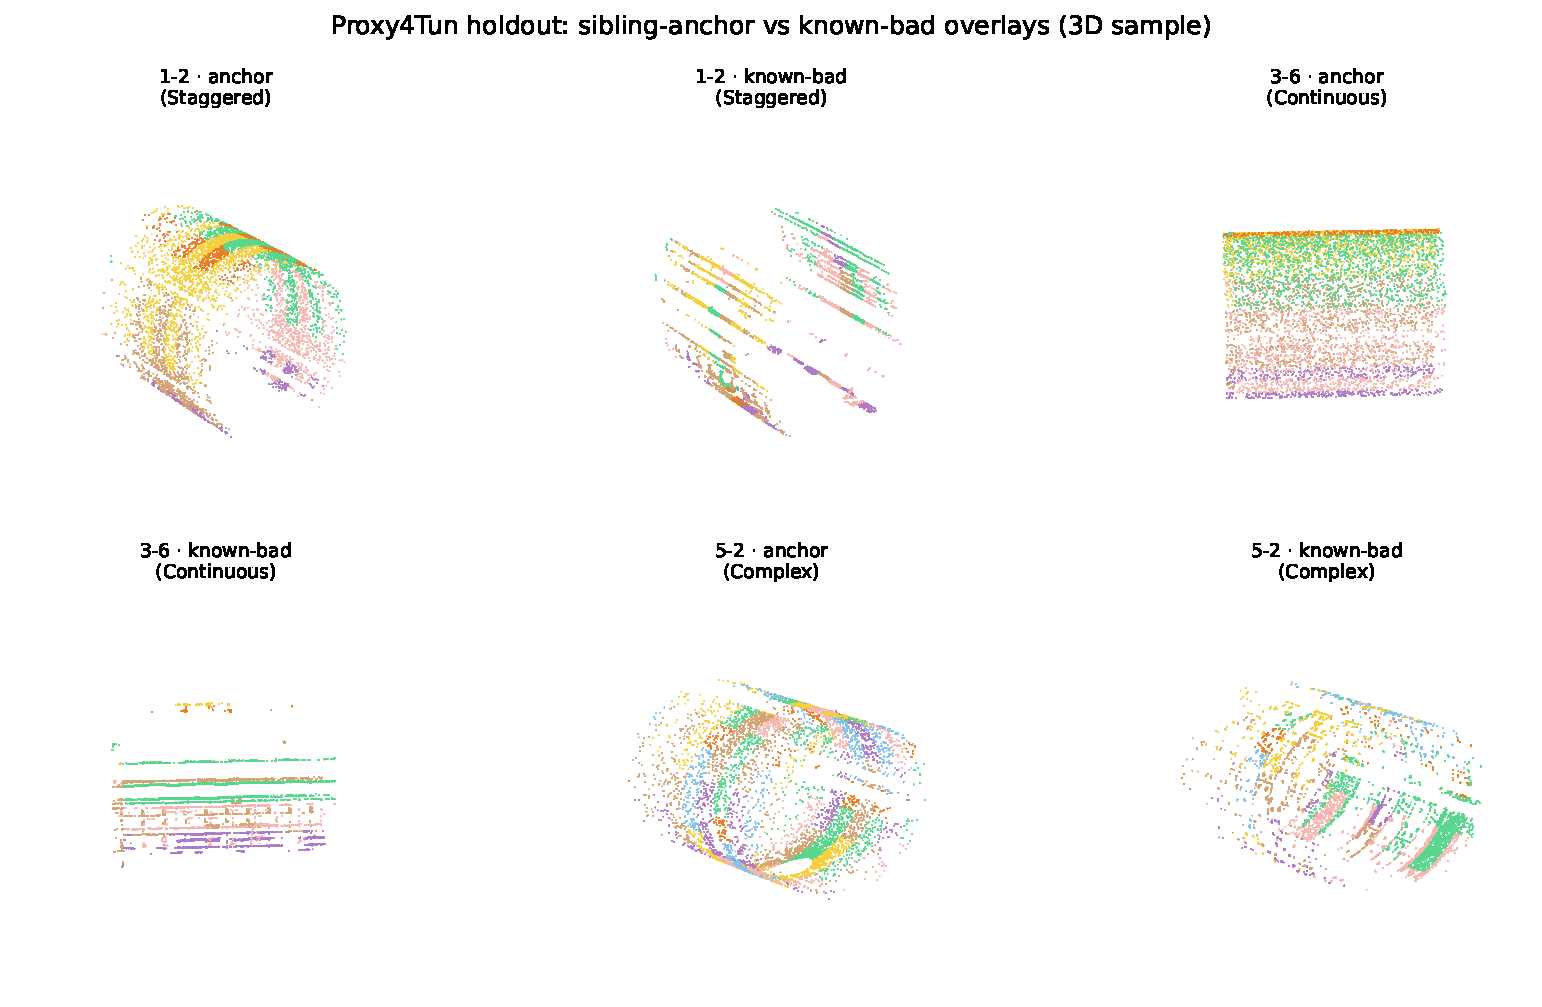
\includegraphics[width=0.98\textwidth]{figures/proxy4tun_3d_anchor_vs_bad.pdf}
\caption{Qualitative 3D samples on held-out subsets (staggered, continuous,
complex). Top: sibling-anchor configurations. Bottom: family known-bad
configurations. Points coloured by predicted segment class (background
suppressed). The proxy separates these regimes without access to labels.}
\label{fig:3d-anchor-bad}
\end{figure*}

\textbf{Blocking low-quality runs.} Used as an alarm at threshold
$\tau = 0.495$, the proxy flags all 27 known-bad runs while raising no false
alarms on the 27 sibling-anchor runs (Table~\ref{tab:holdout-fidelity});
anchor-versus-bad ranking is correct on all 27 subset pairs
(Fig.~\ref{fig:3d-anchor-bad} shows representative pairs). Given the size of
the flagged set we report raw counts rather than rates; the operating point
was fixed before holdout scoring and not tuned on the test subsets.

In practical terms, scoring a run is a five-feature linear evaluation over
artifacts the pipeline has already produced --- effectively free relative to
the pipeline run itself, and requiring no annotation. This is what makes the
proxy usable as an always-on acceptance gate and as a between-round selection
signal for iterative refinement (Section~\ref{sec:poc-verification}).
